\section{Data Processing}
% Delete the text and write your Results here:
%------------------------------------
The dataset of cats and dogs are compromised of 25000 images that are 400 by 500 photos. \par
The first step of generating the training data is grayscaling it. Grayscaling is done by OpenCV's IMREAD\_GRAYSCALE option. \par
\begin{figure}
    \centering
    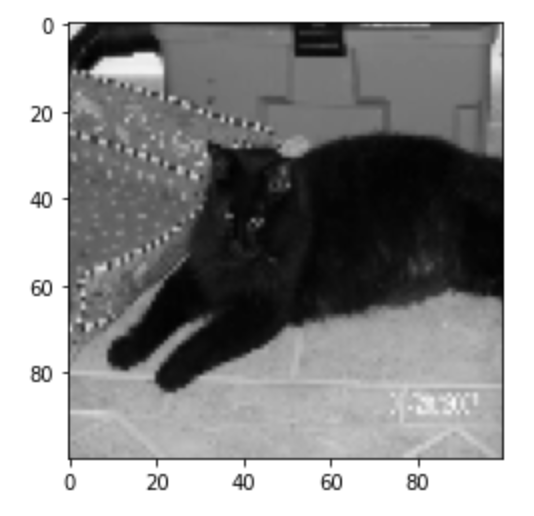
\includegraphics[width=0.48\textwidth]{Images/cat_subres.png}
    \caption{A gray and white, subsampled photo of a cat}
    \label{fig:cat_subres}
\end{figure}
After grayscaling the images, the next step is resizing it. For resizing, a 128 by 128 resolution were chosen, because it was the better resolution for quality and size. The resizing task was also done by OpenCV. \par
Processed dataset is split by 90\% train and 10\% test for checking the accuracies of each network and their one zero losses. \par
After these steps, the images are saved to use in our training and foldings. 